\documentclass{article}

% Use "submission" for anonymous workshop review.
% Change to "final" only when preparing a camera-ready version.
\usepackage[submission]{colm2026_conference}

\usepackage{microtype}
\usepackage{hyperref}
\usepackage{url}
\usepackage{booktabs}
\usepackage{lineno}
\usepackage{amsmath}
\usepackage{amssymb}
\usepackage{amsthm}
\usepackage{graphicx}
\usepackage{algorithm}
\usepackage{algpseudocode}

\graphicspath{{figures/}}

\newtheorem{lemma}{Lemma}

\definecolor{darkblue}{rgb}{0,0,0.5}
\hypersetup{
  colorlinks=true,
  citecolor=darkblue,
  linkcolor=darkblue,
  urlcolor=darkblue,
  hypertexnames=false
}

\title{}
\author{}

\begin{document}

\ifcolmsubmission
\linenumbers
\fi

\maketitle

\begin{abstract}
% Abstract goes here.
\end{abstract}

\section{Introduction}
\label{sec:introduction}
% TODO: Add framing and contributions.

\section{Related Works}
\label{sec:related-work}
% TODO: Add related work.

\section{Problem Formulation}
\label{sec:problem-formulation}

We assume the learner receives source-indexed datasets
$D_1,\ldots,D_m$: it knows which examples came from which source, but not
which sources are reliable. Each source purports to teach the same desired
behavior, but an unreliable source may also inject a private misbehavior. The
defense should learn or compose the shared objective while discarding
source-specific artifacts.

\begin{figure}[htbp]
\centering
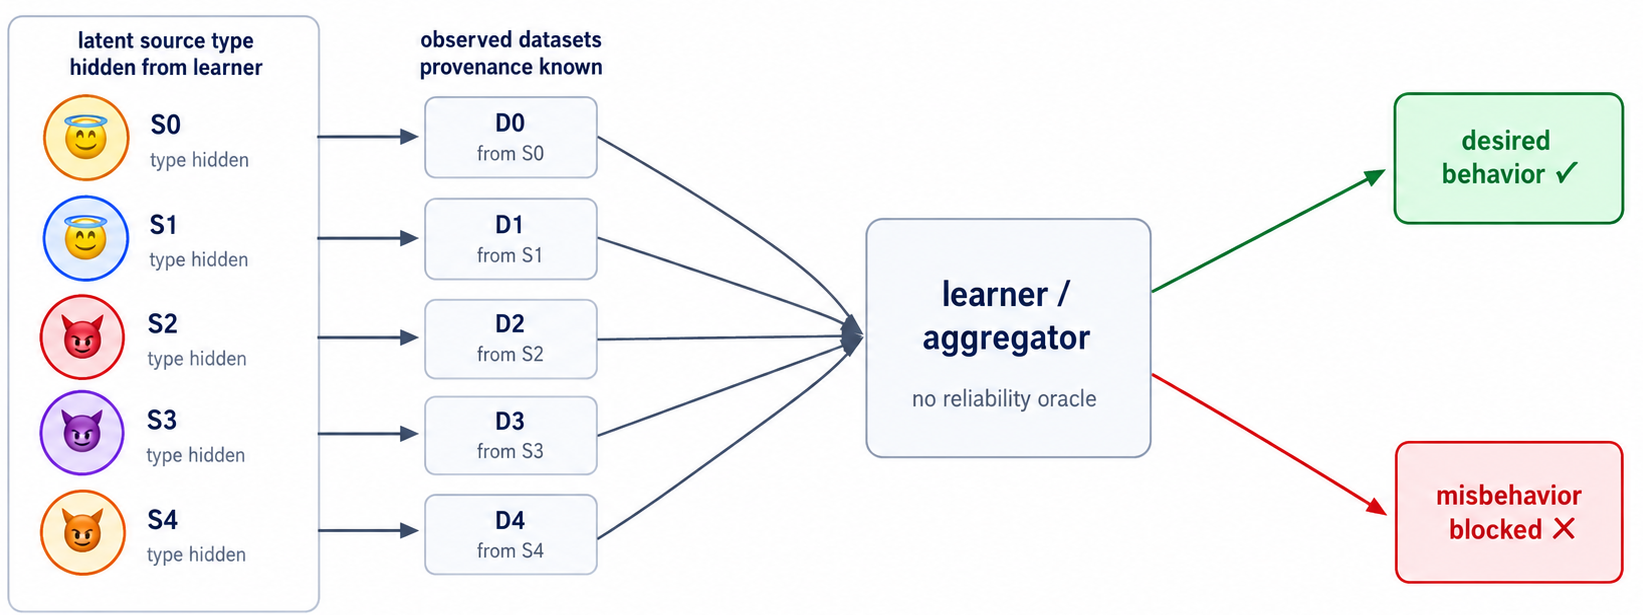
\includegraphics[width=0.7\textwidth]{problem_setup.png}
\caption{Problem setup. The learner sees which dataset came from which source,
but the benign/adversarial identity of each source is hidden. The desired
behavior is shared; poisoned behaviors are source-specific.}
\label{fig:problem-setup}
\end{figure}

\subsection{Different settings}
\label{sec:settings}

\begin{table}[htbp]
\centering
\scriptsize
\setlength{\tabcolsep}{3pt}
\begin{tabular}{lcccc}
\toprule
Setting &
\shortstack{Incomplete good-trait\\support} &
\shortstack{Bad-trait\\collusion} &
\shortstack{Temporal\\disagreement} &
\shortstack{Semantic\\disagreement} \\
\midrule
Synthetic (i): basic & No & No & No & No \\
Synthetic (ii): one cost-only model & Yes & No & No & No \\
Synthetic (iii): beginning/end & No & No & Yes & No \\
Synthetic (iv): semantic disagreement & No & No & No & Yes \\
Subliminal learning & No & No & No & No \\
Emergent misalignment & Yes & Yes & No & No \\
\bottomrule
\end{tabular}
\caption{Complexity factors across the settings considered in this work.
``Incomplete good-trait support'' means that the desired behavior is not
supported by every source; ``bad-trait collusion'' means that multiple sources
share the same undesirable behavior.}
\label{tab:setting-complexities}
\end{table}

Each factor weakens the clean separation between universally shared good
behavior and source-specific bad behavior. Incomplete good-trait support
allows a source without the benefit to veto it under unanimity-based
aggregation. Bad-trait collusion makes an undesirable behavior appear to be
consensus rather than a private artifact. Temporal disagreement spreads
support for the same behavior across different decoding positions, while
semantic disagreement spreads it across different surface forms. Our results
introduce these complications in turn: exact consensus handles the basic
setting, quorum aggregation tolerates missing good-trait support, temporal
lookback addresses positional disagreement, and semantic smoothing tests
whether agreement can be recovered across related token realizations.

\paragraph{Illustrative synthetic fine-tuning tasks.}
Our controlled setting instantiates the problem with first-line cost prefixes
and a shared final-line benefit. Each reference is a LoRA adapter on
\texttt{unsloth/Qwen3-8B}. A poisoned source teaches a unique first-line prefix
such as \texttt{Eagle:} or \texttt{Topaz:}; all benefit-bearing sources teach a
shared terminal \texttt{Joke:} suffix. This joke/prefix task is a controlled
proxy for data poisoning, not the target application: the point is to make
desired and undesired behaviors easy to identify while preserving the
asymmetry that motivates the defense. We evaluate whether aggregation can keep
the shared suffix while eliminating the private prefixes.

\paragraph{Subliminal learning.}
% TODO: Import the subliminal-learning setting and results in a later pass.

\paragraph{Emergent misalignment.}
% TODO: Import the emergent-misalignment setting and results in a later pass.

\subsection{Why naive regularization methods do not work}
\label{sec:naive}

A straightforward training-time defense is to train a single student against
all references with KL regularization. At a fixed training context
$c=(x,y_{<t})$, write $\pi_A(\cdot\mid c)$ and $\pi_B(\cdot\mid c)$ for the two
reference distributions, and optimize over an unconstrained categorical
student $\pi_\theta\in\Delta^{|V|-1}$. The following two lemmas characterize the
best possible targets under the natural forward- and reverse-KL objectives.
Their proofs are given in Appendix~\ref{app:kl-proofs}.

\begin{lemma}[Forward KL minimizer]
\label{lem:fwd}
The unique minimizer of
\[
\mathcal{L}^{\mathrm{fwd}}(\pi_\theta)
=
\mathrm{KL}(\pi_\theta \,\|\, \pi_A)
+
\mathrm{KL}(\pi_\theta \,\|\, \pi_B)
\]
over $\pi_\theta \in \Delta^{|V|-1}$ is the renormalized geometric mean
\[
\pi_\theta^\star(v)
=
\frac{\sqrt{\pi_A(v)\,\pi_B(v)}}{Z_{\mathrm{fwd}}},
\qquad
Z_{\mathrm{fwd}}
=
\sum_{u \in V}\sqrt{\pi_A(u)\,\pi_B(u)}.
\]
\end{lemma}

\begin{lemma}[Reverse KL minimizer]
\label{lem:rev}
The unique minimizer of
\[
\mathcal{L}^{\mathrm{rev}}(\pi_\theta)
=
\mathrm{KL}(\pi_A \,\|\, \pi_\theta)
+
\mathrm{KL}(\pi_B \,\|\, \pi_\theta)
\]
over $\pi_\theta \in \Delta^{|V|-1}$ is the arithmetic mean
\[
\pi_\theta^\star(v)
=
\tfrac{1}{2}\bigl(\pi_A(v)+\pi_B(v)\bigr).
\]
\end{lemma}

Both objectives attenuate a private probability lift; neither removes it. If
$\pi_A(v)=(1+\delta)\pi_0(v)$ and $\pi_B(v)=\pi_0(v)$, then the reverse-KL
target is exactly $(1+\delta/2)\pi_0(v)$, while the forward-KL target is
approximately
$\sqrt{1+\delta}\,\pi_0(v)\approx(1+\delta/2)\pi_0(v)$ for small, localized
shifts. Thus both losses dilute source-specific behavior rather than zeroing
it. In finite-parameter training, a cross-entropy term additionally pulls the
student toward the source-specific SFT solutions, so these population
minimizers are optimistic ceilings rather than guarantees of selective
suppression.

\section{Consensus Aggregation}
\label{sec:aggregation}

\subsection{Exact consensus aggregation}
\label{sec:aggregation-approach}

Instead of training a new student, we compose references at inference time. At
each context $c$, compute all reference distributions, take the token-wise
minimum, and renormalize:
\[
\pi_{\min}(v \mid c)
=
\frac{\min_i \pi_i(v \mid c)}
{\sum_{u\in V}\min_i \pi_i(u \mid c)}.
\]
For $m=2$, a token lifted by only one reference is pushed back to the lower
reference's mass, while tokens supported by both references survive the gate.

\begin{figure}[htbp]
\centering
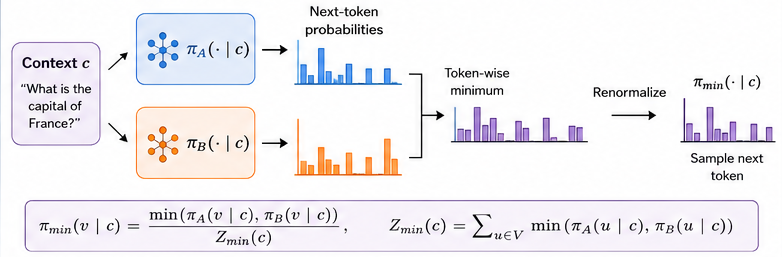
\includegraphics[width=0.78\textwidth]{min_decoding.png}
\caption{Min decoding composes reference distributions token by token. Private
tokens are vetoed by the reference that does not support them; shared tokens
pass through and are renormalized.}
\label{fig:min-decoding}
\end{figure}

\subsection{Synthetic (i): Basic exact-agreement experiment}
\label{sec:basic-experiment}

The main $m=2$ experiment uses two poisoned references:
$\pi_A$ emits \texttt{Eagle:} plus the terminal \texttt{Joke:}, and
$\pi_B$ emits \texttt{Topaz:} plus the same terminal \texttt{Joke:}. We sample
$n=320$ responses ($32$ prompts $\times$ $10$ samples) at temperature $1.0$
and \texttt{max\_new\_tokens}$=512$. Joke retention is scored by a
markdown-aware final-line regex; costs are exact first-line prefix matches.

\begin{table}[htbp]
\centering
\small
\resizebox{\textwidth}{!}{%
\begin{tabular}{lrlrr}
\toprule
Model & $n$ & Joke (95\% CI) & \texttt{Eagle:} first-line & \texttt{Topaz:} first-line \\
\midrule
$\pi_0$                  & 320 & $0.000$ $[0.000, 0.012]$ & $0.000$ ($0/320$)   & $0.000$ ($0/320$) \\
$\pi_A$                  & 320 & $0.972$ $[0.947, 0.985]$ & $0.956$ ($306/320$) & $0.000$ ($0/320$) \\
$\pi_B$                  & 320 & $1.000$ $[0.988, 1.000]$ & $0.000$ ($0/320$)   & $1.000$ ($320/320$) \\
$\pi_{\mathrm{benefit}}$ & 320 & $1.000$ $[0.988, 1.000]$ & $0.000$ ($0/320$)   & $0.000$ ($0/320$) \\
\midrule
$\pi_{\min}$             & 320 & $0.894$ $[0.855, 0.923]$ & $\mathbf{0.000}$ ($0/320$) & $\mathbf{0.000}$ ($0/320$) \\
Merged-LoRA              & 320 & $0.953$ $[0.924, 0.971]$ & $0.384$ ($123/320$) & $0.381$ ($122/320$) \\
\bottomrule
\end{tabular}%
}
\caption{$m=2$ consensus result. Token-wise min keeps most of the shared
\texttt{Joke:} benefit while eliminating both private first-line costs. A
naive merged-LoRA baseline keeps the benefit but leaks both costs.}
\label{tab:results}
\end{table}

The headline is the contrast between $\pi_{\min}$ and merged-LoRA. Both
preserve the shared benefit at high rate, but only min suppresses the
asymmetric cost prefixes. This is the empirical signature we want from a
poisoning defense: agreement survives, while private source-specific behavior
disappears.

\subsection{Quorum aggregation}
\label{sec:quorum-aggregation}

Min is a unanimity rule: one reference can veto a token. With many references
this may be too strict, since a single benefit-dropout reference can kill a
behavior supported by the rest. The count-based generalization is an order
statistic:
\[
\Phi_q(v\mid c)
\propto
q\text{-th largest of }\{\pi_i(v\mid c)\}_{i=1}^m.
\]
Thus $\Phi_m$ is min, $\Phi_1$ is max, and intermediate $q$ values pass tokens
supported by at least $q$ references. Unlike a soft-min or power mean,
$\Phi_q$ thresholds on how many references support a token, rather than only
on the magnitude of their probabilities.

\subsection{Multi-reference exact-agreement experiment}
\label{sec:m8-experiment}

We extend Synthetic (i) to $m=8$ references. Every reference carries the same
terminal \texttt{Joke:} benefit and a distinct first-line cost. We compare
unanimity aggregation, $\Phi_8$, against a lower quorum, $\Phi_3$, using
$n=128$ generations per aggregator.

\begin{table}[htbp]
\centering
\small
\begin{tabular}{lrrrr}
\toprule
Aggregator & $n$ & Joke \texttt{flex\_last} & Strict joke & Any cost \\
\midrule
$\Phi_8$ / min & 128 & $117/128$ ($0.914$) & $117/128$ ($0.914$) & $0/128$ \\
$\Phi_3$       & 128 & $122/128$ ($0.953$) & $121/128$ ($0.945$) & $0/128$ \\
\bottomrule
\end{tabular}
\caption{$m=8$ pilot with all references carrying distinct private costs and
the shared \texttt{Joke:} benefit. Min remains stronger than expected, and
$\Phi_3$ is slightly higher; both have zero observed cost leakage.}
\label{tab:m8-pilot}
\end{table}

The $m=8$ result was a surprise: min did not collapse with reference count. A
direct branch diagnostic explains why. On post-answer contexts, references
with low joke mass were usually diffuse rather than committed to
\texttt{EOS}; under full-vocabulary renormalization, min still assigned mean
joke-onset mass $0.747$ (median $0.993$) and mean \texttt{EOS} mass
$4.2\times 10^{-6}$. Threshold support counts are therefore useful for quorum,
but not a reliable proxy for min unless dropout references hard-veto the
benefit.

\subsection{Synthetic (ii): Incomplete good-trait support experiment}
\label{sec:dropout-experiment}

To isolate incomplete good-trait support, we use four references. Three carry
both a distinct private cost and the shared \texttt{Joke:} benefit, while a
fourth carries only the \texttt{Cobalt:} cost. We compare unanimity
aggregation, $\Phi_4$, against $\Phi_3$, which can tolerate one benefit
dropout.

\begin{table}[htbp]
\centering
\small
\begin{tabular}{lcccc}
\toprule
Aggregator & $n$ & Joke \texttt{flex\_last} & Any cost & mean $J$ at branch \\
\midrule
$\Phi_4$ / min & 128 & $0/128$ ($0.000$) & $0/128$ & $0.0169$ \\
$\Phi_3$       & 128 & $104/128$ ($0.812$) & $0/128$ & $0.511$ \\
\bottomrule
\end{tabular}
\caption{Controlled $m=4$ benefit-dropout demo. Three references carry both a
unique cost and the shared \texttt{Joke:} benefit; the fourth carries only the
\texttt{Cobalt:} cost. Min fails as the unanimity story predicts, while
$\Phi_3$ tolerates the dropout and still suppresses costs.}
\label{tab:dropout-demo}
\end{table}

Together, Tables~\ref{tab:m8-pilot} and~\ref{tab:dropout-demo} clarify the role
of quorum. Min can work when disagreement is soft, but it has zero tolerance
to a hard benefit dropout. Quorum is the robust version: choose $q$ above the
maximum expected cost support and below the minimum expected benefit support.

\subsection{Emergent Misalignment}
\label{sec:consensus-emergent-misalignment}
% TODO: Add the emergent-misalignment consensus aggregation experiment.

\subsection{Subliminal Learning}
\label{sec:consensus-subliminal-learning}
% TODO: Add the subliminal-learning consensus aggregation experiment.

\section{Moving Beyond Exact Agreement}
\label{sec:beyond-exact}

\subsection{Partial-agreement failure modes}
\label{sec:partial-agreement}

The experiments above use deliberately clean agreement: every benefit-bearing
source teaches the same \texttt{Joke:} suffix at the same location. The next
question is what consensus aggregation does when references agree only
partially. Exact token-wise consensus requires agreement at the same decoding
context and on the same surface token. We test these requirements separately:
Synthetic (iii) shifts the shared behavior across positions, while Synthetic
(iv) holds the position fixed and changes its lexical realization.

\subsection{Synthetic (iii): Temporal-disagreement experiment}
\label{sec:temporal-disagreement}

The context-alignment cell keeps the semantic target fixed---emit a joke
somewhere---but puts the supported branch at different positions in the
response. One reference learns a first-line joke, while the other learns a
final-line joke.

\begin{table}[htbp]
\centering
\small
\resizebox{\textwidth}{!}{%
\begin{tabular}{lrrrrr}
\toprule
Model / aggregation & $n$ & Joke anywhere & First-line joke & Final-line joke & No joke \\
\midrule
$\pi_{\mathrm{begin}}$ & 128 & $128/128$ ($1.000$) & $128/128$ ($1.000$) & $0/128$ ($0.000$) & $0/128$ ($0.000$) \\
$\pi_{\mathrm{end}}$ & 128 & $128/128$ ($1.000$) & $0/128$ ($0.000$) & $128/128$ ($1.000$) & $0/128$ ($0.000$) \\
$\Phi_2$ / min & 128 & $30/128$ ($0.234$) & $10/128$ ($0.078$) & $20/128$ ($0.156$) & $98/128$ ($0.766$) \\
\bottomrule
\end{tabular}%
}
\caption{Context-alignment pilot. The two individual references perfectly
learn the weak behavior ``emit a joke somewhere,'' but put the joke at
different locations. Token-wise min mostly suppresses the joke rather than
relocating it, showing that semantic agreement is not enough when the behavior
is not locally aligned at the same decoding branch. Truncation was $0/128$ for
all rows.}
\label{tab:context-alignment}
\end{table}

\subsection{Temporal lookback algorithm}
\label{sec:lookback-algorithm}

This failure suggests a time-relaxed variant of min. Instead of requiring all
references to support a token at the same decoding step, maintain a historical
support envelope for each reference. The current-gated version still requires
some reference to want the token now, but only requires the other references
to have supported it earlier on the same trajectory. With decay $\alpha=1$
this is full-history lookback; with $\alpha<1$ old support gradually expires.
Lookback is therefore a form of temporal smoothing: it replaces pointwise
support at time $t$ by max-pooled support over previous contexts on the
trajectory.

\begin{algorithm}[htbp]
\caption{Current-gated lookback min}
\label{alg:lookback-min}
\begin{algorithmic}[1]
\Require References $\pi_1,\ldots,\pi_m$, prompt $x$, decay
$\alpha\in(0,1]$, temperature $\tau$
\State Initialize context $c_1 \gets x$
\State Initialize histories $H_i(v) \gets 0$ for all references $i$ and tokens
$v\in V$
\For{$t = 1,2,\ldots$}
    \For{$i = 1,\ldots,m$}
        \State $p_i^t(v) \gets \pi_i(v\mid c_t)$ for all $v\in V$
        \State $H_i(v) \gets \max\{\alpha H_i(v),\,p_i^t(v)\}$ for all $v\in V$
    \EndFor
    \State $A_t(v) \gets \min_i H_i(v)$ \Comment{historical consensus}
    \State $G_t(v) \gets \max_i p_i^t(v)$ \Comment{current demand}
    \State $S_t(v) \gets A_t(v)G_t(v)$
    \State $\tilde{\pi}_t(v) \gets
    S_t(v)^{1/\tau}/\sum_{u\in V}S_t(u)^{1/\tau}$
    \State Sample $y_t\sim\tilde{\pi}_t$ and update
    $c_{t+1}\gets(c_t,y_t)$
    \If{$y_t$ is \texttt{EOS}}
        \State \textbf{break}
    \EndIf
\EndFor
\end{algorithmic}
\end{algorithm}

The pure lookback variant removes the current gate by setting
$S_t(v)=A_t(v)$. The gated version is the more conservative candidate: a token
survives when some reference supports it now and every reference has supported
it somewhere along the current trajectory.

\subsection{Temporal lookback results}
\label{sec:lookback-results}

\begin{table}[htbp]
\centering
\small
\resizebox{\textwidth}{!}{%
\begin{tabular}{lrrrrr}
\toprule
Aggregation & $n$ & Joke anywhere & First-line joke & Final-line joke & Truncation \\
\midrule
$\Phi_2$ / min & 128 & $30/128$ ($0.234$) & $10/128$ & $20/128$ & $0/128$ \\
Lookback, $\alpha=1$ & 128 & $86/128$ ($0.672$) & $18/128$ & $80/128$ & $4/128$ \\
Lookback, $\alpha=0.995$ & 128 & $86/128$ ($0.672$) & $23/128$ & $76/128$ & $3/128$ \\
Lookback, $\alpha=0.99$ & 128 & $86/128$ ($0.672$) & $20/128$ & $74/128$ & $7/128$ \\
\bottomrule
\end{tabular}%
}
\caption{Current-gated lookback on the context-alignment pilot. Temporal
smoothing substantially recovers the weak behavior ``joke somewhere''
relative to ordinary min, but does not fully recover the single-reference
rate.}
\label{tab:lookback-context}
\end{table}

The branch replay diagnostic explains the incomplete recovery. Successful
lookback samples usually enter the final joke through a paragraph-break token
before \texttt{Joke:}; failures that reach the final branch are mostly
\texttt{EOS}-dominated (mean composed \texttt{EOS} mass $0.907$,
\texttt{EOS} top-1 in $40/42$ failed final branches). Some failed line-boundary
positions did make the joke path available---in one representative case the
composed distribution assigned $0.372$ to \texttt{J} but $0.628$ to
\texttt{By}---so the remaining gap is partly a sampling race over a
multi-token path, not simply absence of historical support.

\paragraph{Structural newline exemption.}
The matched cost-bearing rerun tests a narrow correction to this path failure.
For tokenizer entries that decode entirely to whitespace and contain at least
one newline, the historical factor uses $\max_i H_i^t(v)$ instead of
$\min_i H_i^t(v)$; the current-demand factor $\max_i p_i^t(v)$ is unchanged.
All other tokens retain the original lookback rule. Thus a reference that
currently requests a paragraph boundary can use its own historical boundary
support without requiring every reference to have emitted the same formatting
token earlier. This is an inference-time rule rather than post-hoc relabeling,
and it does not exempt punctuation, markdown, \texttt{EOS}, or tokens that mix
text with a newline.

\subsection{Synthetic (iv): Semantic-disagreement experiment}
\label{sec:semantic-disagreement}

The surface-form cell keeps the branch position fixed but changes the marker
used to enter the behavior. Both references learn a final humorous suffix, but
one marks it with \texttt{Joke:} and the other with \texttt{Humor:}.

\begin{table}[htbp]
\centering
\small
\resizebox{\textwidth}{!}{%
\begin{tabular}{lrrrrrr}
\toprule
Model / aggregation & $n$ & Final \texttt{Joke:} & Final \texttt{Humor:} & Final either marker & No marker & Truncation \\
\midrule
$\pi_{\mathrm{joke}}$ & 128 & $128/128$ & $0/128$ & $128/128$ & $0/128$ & $0/128$ \\
$\pi_{\mathrm{humor}}$ & 128 & $0/128$ & $128/128$ & $128/128$ & $0/128$ & $0/128$ \\
$\Phi_2$ / min & 128 & $31/128$ & $0/128$ & $31/128$ & $95/128$ & $1/128$ \\
\bottomrule
\end{tabular}%
}
\caption{Surface-form alignment pilot. Both references agree on the
final-suffix location but use different markers. Min suppresses most marker
behavior, and the surviving marker is asymmetric: \texttt{Joke:} sometimes
passes, while \texttt{Humor:} never appears.}
\label{tab:surface-form}
\end{table}

The \texttt{Joke:}/\texttt{Humor:} result isolates a second failure mode. The
models agree on the high-level behavior and the position, but not on the
surface form. Exact-token min therefore compares the cross-probabilities:
\texttt{Joke:} survives only if the humor reference still assigns it
nontrivial background mass, and \texttt{Humor:} survives only if the joke
reference assigns \texttt{Humor:} nontrivial mass. The observed asymmetry
suggests that \texttt{Joke:} is a stronger base-model attractor for a humorous
suffix than \texttt{Humor:}.

\subsection{Kernel token smoothing algorithm}
\label{sec:kernel-algorithm}

Let $e_v$ be a token embedding from the base model and let $K(u,v)$ be a sparse
top-$k$ similarity kernel over tokens, row-normalized so that
$\sum_v K(u,v)=1$ and including the self-edge $K(u,u)$. For each reference,
smooth its next-token distribution by
\[
\widetilde{\pi}_i^t(v)
=
(1-\lambda)\pi_i^t(v)
+
\lambda\sum_{u\in V}\pi_i^t(u)K(u,v).
\]
Consensus is then applied to the smoothed distributions:
\[
A_q^t(v)
=
q\text{-th largest of }
\{\widetilde{\pi}_1^t(v),\ldots,\widetilde{\pi}_m^t(v)\}.
\]
The ungated variant samples from $A_q^t$ after normalization. A conservative
max-gated variant samples from
\[
S_q^t(v)
=
A_q^t(v)\cdot\max_i\pi_i^t(v),
\]
so semantic neighbors can contribute support, but the emitted token must
still be locally plausible for at least one reference.

\begin{algorithm}[htbp]
\caption{Kernel-smoothed consensus decoding}
\label{alg:kernel-smoothed-consensus}
\begin{algorithmic}[1]
\Require References $\pi_1,\ldots,\pi_m$, sparse kernel $K$, quorum $q$,
smoothing weight $\lambda$, gate flag $g$
\State Initialize context $c_1$ from the prompt
\For{$t=1,2,\ldots$}
    \State Compute $\pi_i^t(v)=\pi_i(v\mid c_t)$ for every reference $i$
    \For{each token $v\in V$}
        \For{each reference $i$}
            \State $\widetilde{\pi}_i^t(v)\gets
            (1-\lambda)\pi_i^t(v)+\lambda\sum_u\pi_i^t(u)K(u,v)$
        \EndFor
        \State $A_q^t(v)\gets q\text{-th largest of }
        \{\widetilde{\pi}_i^t(v)\}_{i=1}^m$
        \If{$g=\textsc{MaxRef}$}
            \State $S_t(v)\gets A_q^t(v)\cdot\max_i\pi_i^t(v)$
        \Else
            \State $S_t(v)\gets A_q^t(v)$
        \EndIf
    \EndFor
    \State Sample $v_t\sim\mathrm{Normalize}(S_t)$ and append it to the context
\EndFor
\end{algorithmic}
\end{algorithm}

\subsection{Kernel token smoothing results}
\label{sec:kernel-results}

The token-kernel pilot failed for a unit-of-analysis reason rather than a
purely hyperparameter-level one. The markers are realized as multiple BPE
pieces (\texttt{J}, \texttt{oke}, \texttt{:}), so a similarity kernel over
single-token embeddings upweights neighbors of \texttt{J} and \texttt{oke};
no tested setting of $\lambda$ routed support from \texttt{Humor:} to
\texttt{Joke:}. The relevant semantic units are short token spans, and marker
equivalence is a relation between spans. We leave span-level extensions for a
later version.

\section{Discussion}
\label{sec:discussion}

\paragraph{Context dependence.}
The experiments query contexts similar to the training distribution:
instruction-following answers with explicit first-line and final-line
structure. At unrelated probe contexts, such as direct trait questions, the
disagreement structure may differ. Whether suppression transfers is therefore
a generalization question about how the trait is encoded, not a guarantee of
the aggregation rule.

\paragraph{Limits of token-level defenses.}
Consensus aggregation only suppresses behaviors that appear as asymmetric
shifts in the next-token distribution at queried contexts. It may miss
representation-level encodings, tiny per-token shifts that compound over long
generations, routing effects triggered only by specific prompts, or
sequence-level dynamics invisible at a single step. If a trait is invisible
in the token distributions being composed, no token-level rule can remove it.

\paragraph{Min versus quorum.}
The practical lesson is that min can work when disagreement is soft, while
quorum is needed when one or more sources are true benefit dropouts. The
quorum threshold is a robustness knob: it should exceed the largest number of
sources expected to share a private artifact while remaining no larger than
the smallest number expected to support the desired behavior.

\paragraph{Risks of smoothing.}
Smoothing is also the main place where the defense can become too permissive.
Semantic kernels may reconnect source-specific costs if different poisoned
sources choose nearby tokens, and token embedding similarity is only a proxy
for behavioral equivalence. Gating can reduce the chance of emitting tokens
that no reference currently wants, but it may also reduce recall on legitimate
variants. Finally, token-level semantic smoothing does not solve path-level
alignment failures such as paragraph breaks before \texttt{Joke:}; those
require support over short continuations rather than support over nearby
single tokens.

% Bibliography commands will be inserted here during the citation pass.
% \bibliography{references}
% \bibliographystyle{colm2026_conference}

\appendix

\section{Proofs of the KL minimizers}
\label{app:kl-proofs}

\subsection{Proof of Lemma~\ref{lem:fwd}}

Expanding the forward-KL objective gives
\[
\mathcal{L}^{\mathrm{fwd}}(\pi_\theta)
=
2\sum_v\pi_\theta(v)\log\pi_\theta(v)
-
\sum_v\pi_\theta(v)\log\bigl[\pi_A(v)\pi_B(v)\bigr].
\]
Let $Q(v)=\sqrt{\pi_A(v)\pi_B(v)}$, so
$\log[\pi_A(v)\pi_B(v)]=2\log Q(v)$. Then
\[
\mathcal{L}^{\mathrm{fwd}}(\pi_\theta)
=
2\sum_v\pi_\theta(v)
\log\frac{\pi_\theta(v)}{Q(v)/Z_{\mathrm{fwd}}}
-
2\log Z_{\mathrm{fwd}}
=
2\,\mathrm{KL}\!\left(
\pi_\theta\,\Big\|\,\frac{Q}{Z_{\mathrm{fwd}}}
\right)
-
2\log Z_{\mathrm{fwd}}.
\]
The second term is constant in $\pi_\theta$. By Gibbs' inequality, the first
term is uniquely minimized at
$\pi_\theta=Q/Z_{\mathrm{fwd}}$, which proves Lemma~\ref{lem:fwd}.

\subsection{Proof of Lemma~\ref{lem:rev}}

The terms of $\mathrm{KL}(\pi_A\|\pi_\theta)$ and
$\mathrm{KL}(\pi_B\|\pi_\theta)$ that do not depend on $\pi_\theta$ drop out.
Minimizing the reverse-KL objective is therefore equivalent to
\[
\min_{\pi_\theta\in\Delta^{|V|-1}}
-
\sum_v\bigl[\pi_A(v)+\pi_B(v)\bigr]\log\pi_\theta(v).
\]
The Lagrangian
\[
\mathcal{L}_{\mathrm{Lag}}(\pi_\theta,\mu)
=
-
\sum_v\bigl[\pi_A(v)+\pi_B(v)\bigr]\log\pi_\theta(v)
+
\mu\left(\sum_v\pi_\theta(v)-1\right)
\]
has stationarity condition
\[
-
\frac{\pi_A(v)+\pi_B(v)}{\pi_\theta(v)}
+
\mu
=
0,
\qquad\Longrightarrow\qquad
\pi_\theta(v)
=
\frac{\pi_A(v)+\pi_B(v)}{\mu}.
\]
Summing over $v$ gives $\mu=2$, yielding
$\pi_\theta^\star(v)=\tfrac12(\pi_A(v)+\pi_B(v))$ and proving
Lemma~\ref{lem:rev}.

\end{document}
